\chapter{Конструкторский раздел}

\section{Комбинированный алгоритм}
С учетом выявленных недостатков пошагового и событийного алгоритмов предлагается реализовать комбинированный алгоритм таким образом, чтобы на пиковых интервалах он приближался к пошаговому алгоритму, а в промежуточных --- к событийному с большим шагом. Таким образом, проблема неэффективности пошагового алгоритма решается использованием подхода событийного алгоритма на промежуточных интервалах. Однако для решения проблем событийного алгоритма, а именно --- растущей сложности операций вставки и получения событий в список будущих событий, необходимо реализовать структуру для хранения событий более эффективным способом.

\section{Часовая структура данных}
Предлагается реализовать структуру данных для хранения событий, сложность операций вставки и получения элементов для которой будет составлять $O(1)$.

На рисунке \ref{img:hybrid_structure} представлена разработанная для этой задачи структура данных. В основу положена идея об иерархической системе контроля времени, управляемой событиями (HECTAS) \cite{system_modelling_eng}.

\begin{figure}[h!btp]
	\centering
	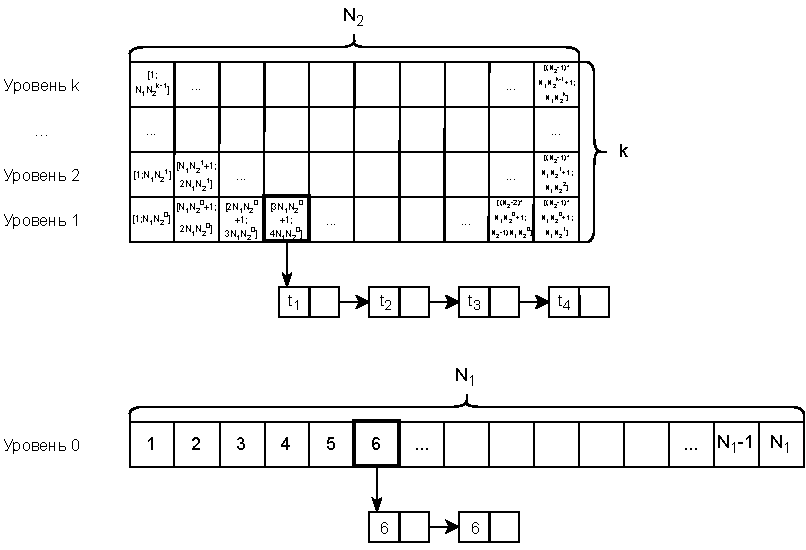
\includegraphics[width=1\columnwidth]{inc/img/hybrid_structure.pdf}
	\caption{Часовая структура данных для хранения событий}
	\label{img:hybrid_structure}	
\end{figure}

Часовая структура представлена многоуровневой системой списков событий. Каждая ячейка системы --- связный список событий. 

Нулевой уровень представлен массивом таких списков и имеет длину $N_1$. События, попадая на нулевой уровень, обрабатываются аналогично пошаговому алгоритму: временной шаг между соседними ячейками равен минимальному тику таймера модельного времени (единице). Для оптимального моделирования системы с квазисинхронным распределением рекомендуется подобрать длину нулевого уровня таким образом, чтобы она покрывала максимальную длину пиковых интервалов.

Ненулевые уровни системы объединены в массив, каждый уровень, аналогично нулевому, представлен массивом списков событий с фиксированной длиной $N_2$, отличной от длины нулевого уровня (совпадение размерностей допустимо). Для удобства массив уровней будет называться далее таблицей событий. Первая ячейка каждого уровня таблицы описывает временной диапазон от 1 до максимального значения предыдущего уровня. Временной шаг на каждом уровне (гранулярность уровня) совпадает с вместимостью предыдущего уровня.

Гранулярность уровня можно рассчитать по формуле:
\begin{equation}
	G(\text{level}) = 
	\begin{cases}
		1 & \text{, level = 0,} \\
		N_1 N_2^{\text{level}-1} & \text{, иначе,}
	\end{cases}
\end{equation}
где: \\
$N_1$ --- размер нулевого уровня часовой структуры, \\
$N_2$ --- размер табличного уровня часовой структуры. \\ \\


%Обход такой структуры при моделировании системы начинается с верхнего уровня таблицы. В случае обнаружения событий в текущей ячейке таблицы происходит спуск по таблице событий: обнаруженные события размещаются в ячейках предыдущего уровня, после чего происходит аналогичный обход

Необходимое количество уровней в зависимости от требуемого времени моделирования может быть рассчитано по формуле:
\begin{equation}
	k(\text{maxTime}) = \frac{\text{maxTime}} {N_1} \text{,}	\\
\end{equation}
где: \\
maxTime --- общее время моделирования системы. \\ \\

Для вставки события в часовую структуру необходимо рассчитать столбец и уровень нужной ячейки. Нумерация столбцов начинается с 1, как и нумерация уровней в таблице.

Для определения уровня, в который нужно поместить новое событие, необходимо воспользоваться следующей формулой:

\begin{equation}
	\text{Level}(\text{time}) =  \lceil \log_{N_2} \frac{\text{time}}{N_1} \rceil \text{,} \\
\end{equation}
где: \\
time --- время возникновения события. \\ \\

Для определения столбца, в который нужно поместить новое событие, необходимо предварительно определить уровень, после чего воспользоваться следующей формулой:

\begin{equation}
	\text{Column(time, level)} = 
	\begin{cases}
		(\text{time} - 1) \mod N_1 + 1 & \text{, level = 0,} \\
		\lceil \frac{\text{time}}{G(\text{level})} \rceil & \text{, иначе,}
	\end{cases}
	\label{eq:column}
\end{equation}
где: \\
$N_1$ --- размер нулевого уровня часовой структуры, \\
$G(\text{level})$ --- гранулярность уровня level. \\ \\

Подбор значений $N_1$ и $N_2$ зависит от требований, предъявляемых к моделируемой системе. Как уже говорилось ранее, в случае квазисинхронного распределения в системе значение $N_1$ следует подобрать таким образом, чтобы оно покрывало максимальный размер пикового интервала. Для $N_2$ же наиболее оптимальным значением будет 10: ввиду множества операций взятия логарифма по основанию $N_2$ возможно использование оптимизированных реализаций взятия десятичного алгоритма. Очевидно, при увеличении обоих величин масштабирование времени в часовой структуре будет больше, что приведет к уменьшению количества уровней в таблице и, как следствие, к уменьшению операций, связанных с перемещением списков событий с одного уровня на другой.


Для наглядности на рисунке \ref{img:hybrid_structure_example} приведен пример заполненной часовой структуры с размеров нулевого уровня $N_1 = 15$, размером табличного уровня $N_2 = 10$ и количеством уровней таблицы $k = 3$.

\begin{figure}[h!btp]
	\centering
	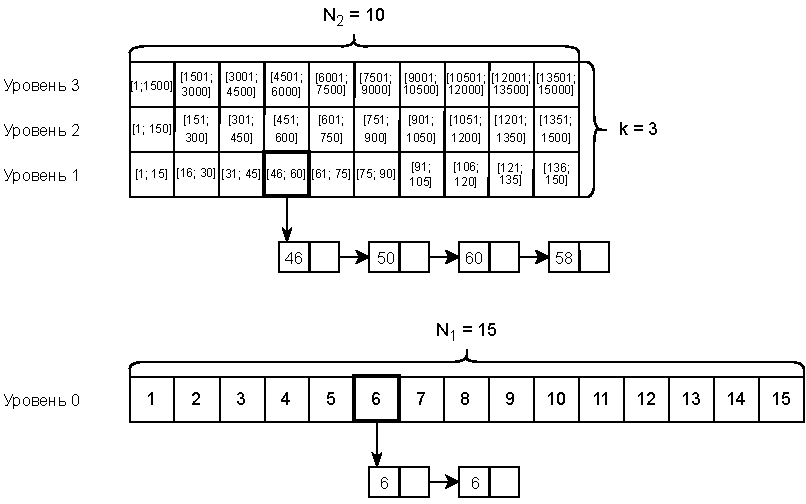
\includegraphics[width=1\columnwidth]{inc/img/hybrid_structure_example.pdf}
	\caption{Часовая структура данных для хранения событий}
	\label{img:hybrid_structure_example}	
\end{figure}

Видно, насколько сильно масштабируется время на верхних уровнях даже при такой небольшой размерности $N_1$. Если при тех же $k$ и $N_2$ взять $N_1$ равным, например, 100, то максимальное время моделирования, описываемое такой структурой, будет достигать 1 млн тиков таймера модельного времени.

\section{Описание алгоритма}
Прежде всего необходимо инициализировать часовую структуру в соответствии с требованиями, предъявляемыми к моделируемой системе. Оптимальный подбор значений описан в предыдущем пункте.

При дальнейшем описании алгоритма будет называть генератором блок системы, который генерирует заявки, а процессором --- блок, который обрабатывает заявки.


Перед началом процесса моделирования необходимо <<запустить>> все генераторы системы, т.е. начать генерацию заявок и поместить в часовую структуру события, связанные с окончанием генерации этих заявок.
На этом этапе (инициализации) события помещаются в ячейки верхнего уровня таблицы событий, однако все последующие события, сгенерированные блоками моделируемой системы размещаются либо в ячейке нулевого уровня, либо в таблице событий, в зависимости от текущего времени и времени возникновения события.


Процесс моделирования представляет собой рекурсивный обход уровней часовой структуры и начинается с верхнего уровня. Текущая ячейка проверяется на наличие событий: если события не найдены, текущее значение таймера увеличивается на гранулярность текущего уровня, иначе начинается обработка списка событий.

Обработка списка событий заключается в последовательном <<спуске>> всех событий на уровень ниже до тех пор, пока не будет достигнут нулевой уровень. Для каждого события из рассматриваемого списка происходит пересчет столбца для уровня ниже. Для этого необходимо пересчитать время события в рамках уровня, на который происходит перемещение. Сделать это можно, использовав следующую формулу:

\begin{equation}
	\text{time'}(\text{level}) =  \text{time} \mod G(\text{level}) + 1 {,} \\
\end{equation}
где: \\
time --- время возникновения события, \\
$G(\text{level})$ --- гранулярность уровня, с которого происходит спуск события. \\ \\

Тогда пересчет столбца для уровня ниже может быть осуществлен с помощью формулы \ref{eq:column} как $\text{Column}(\text{time'}, \text{level} - 1)$.

После спуска списка событий по уровню, на который были перемещены события, осуществляется такой же проход, как и по верхнему: в случае нахождения не пустой ячейки происходит последовательный спуск на уровень ниже, а иначе --- продвижение времени на гранулярность текущего уровня.

Обработка каждого события происходит непосредственно на нулевом уровне часовой структуры. Перед тем, как начать обход нулевого уровня, необходимо определить его текущее окончание временного диапазона. Сделать это можно по формуле:

\begin{equation}
	\text{currentEnd} = \text{currentTime} + N_1 {,} \\
\end{equation}
где: \\
currentTime --- текущее значение таймера модельного времени, \\
$N_1 $ --- размер нулевого уровня часовой структуры. \\ \\

Гранулярность нулевого уровня всегда равна минимальному значению тика модельного времени, т.е. 1, так что при обходе нулевого уровня значение таймера модельного времени инкрементируется, аналогично пошаговому алгоритму. Каждая ячейка нулевого уровня проверяется на наличие событий:
если событие найдено, происходит его обработка, иначе --- переход к следующей ячейке с увеличением значения таймера.

При обработке каждого события (окончание генерации заявки и окончание обработки заявки) происходит создание и добавление в часовую структуру новых событий: о следующем окончании генерации и о следующем окончании обработки заявки. При добавлении нового события необходимо прежде всего проверить, есть ли возможность поместить его на нулевом уровне, сравнив значение времени возникновения события со значением текущего окончания временного диапазона, описываемого нулевым уровнем ($currentEnd$). В случае, если время нового события не превышает это значение, новое событие помещается на нулевой уровень в столбец $Column(time, 0)$, иначе для нового события предварительно вычисляется номер уровня, после чего уже рассчитывается номер столбца ячейки таблицы. События, размещенные таким образом на нулевом уровне будут обработаны во время текущего <<пошагового>> прохода.

По завершении обхода нулевого уровня происходит рекурсивный возврат на предыдущие по следованию уровни, после чего аналогично продолжается их обход. В итоге произойдет возврат в уже пустую ячейку верхнего уровня.

Может возникнуть ситуация, при которой по возвращении в ячейку таблицы список событий, содержащийся в этой ячейке все еще будет непустым. Это происходит ввиду генерации новых событий во время обработки уже существующих. Для обработки таких кейсов введена переменная, содержащая количество повторных обработок текущего уровня --- $retries$, значение которой при первичной обработке ячейки равно 0. 

При обработке непустой ячейки таблицы происходит проверка значения переменной $retries$: если оно равно 0 --- ячейка обрабатывается в первый раз, т.е. происходит обычная, описанная выше, обработка списка событий, иначе --- ячейка обрабатывается повторно и прежде, чем приступать к обработке списка событий, необходимо уменьшить текущее значение таймера модельного времени на величину гранулярности обрабатываемого уровня. Это необходимо сделать из-за того, что в таком случае произойдет повторный обход пустых ячеек уже обработанных уровней и, соответственно, ложное увеличение модельного времени.

Процесс моделирования завершается по наступлении максимального времени моделирования: при добавлении события в часовую структуру время события сравнивается с максимальным временем, и, в случае превышения лимита, добавление события не происходит. Таким образом, при наступлении максимального времени моделирования произойдет возврат на верхний уровень таблицы событий и обход пустых ячеек, оставшихся на нем.


Результатом работы такого симулятора является собранная со всех блоков системы статистика:
информация о среднем времени генерации/обработки заявки, общее количество сгенерированных/обработанных заявок и среднее время ожидания заявки для каждого процессора.

\clearpage
На рисунке \ref{img:hybrid_simulate_schema} представлена схема комбинированного алгоритма продвижения модельного времени. Для удобства часовая структура в схемах называется часами.
\begin{figure}[h!btp]
	\centering
	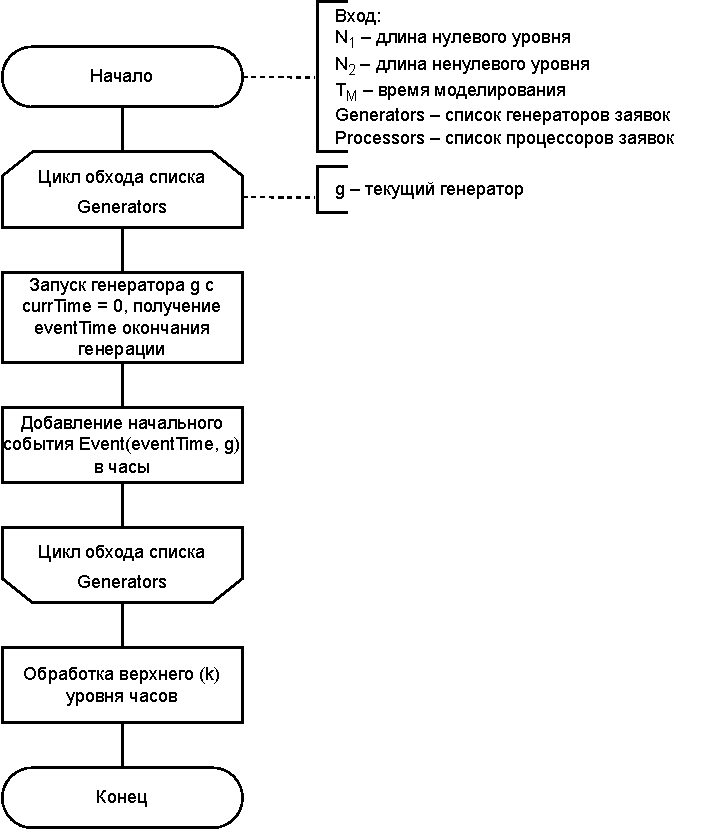
\includegraphics[width=1\columnwidth]{inc/img/hybrid_simulate_schema.pdf}
	\caption{Схема комбинированного алгоритма}
	\label{img:hybrid_simulate_schema}	
\end{figure}

\clearpage
На рисунке \ref{img:hybrid_processLevel_schema} представлена схема алгоритма обработки одного уровня часовой структуры.
\begin{figure}[h!btp]
	\centering
	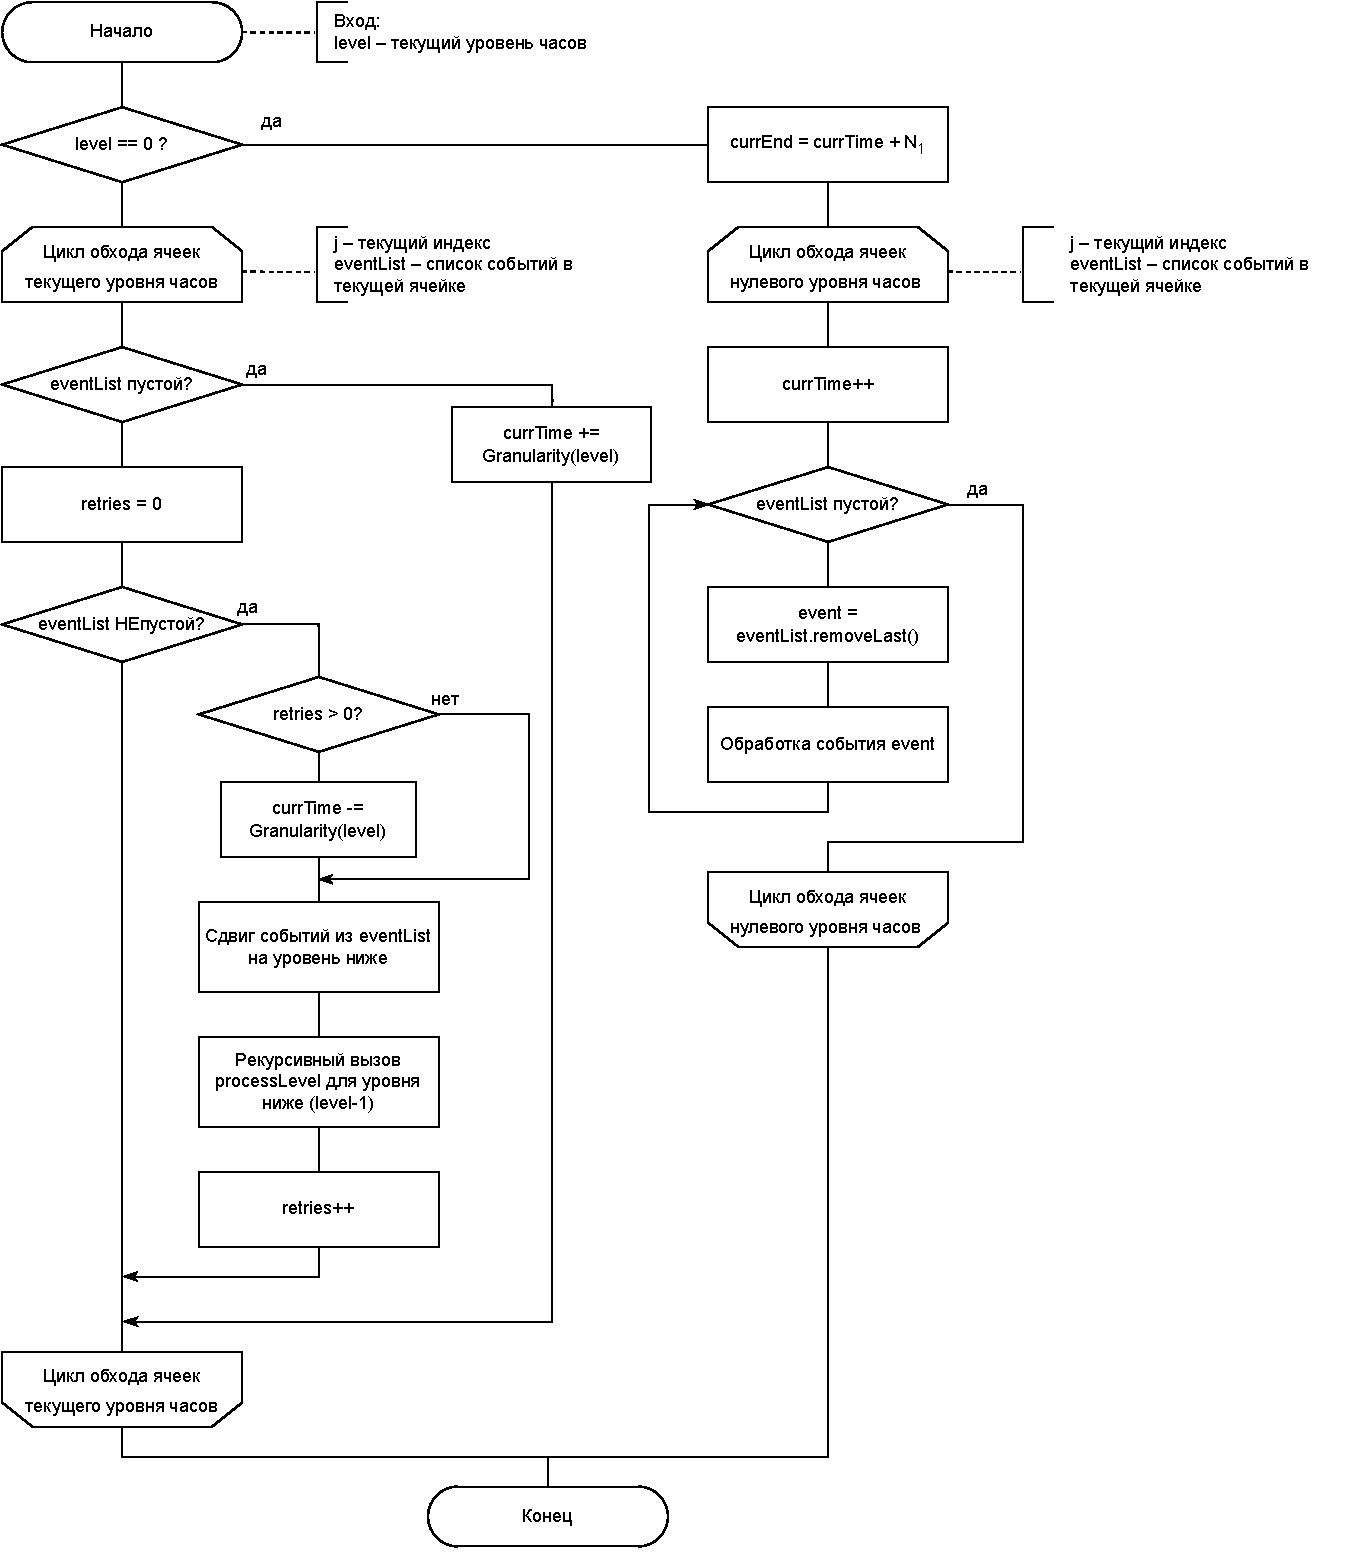
\includegraphics[width=1\columnwidth]{inc/img/hybrid_processLevel_schema.pdf}
	\caption{Схема алгоритма обработки одного уровня часовой структуры}
	\label{img:hybrid_processLevel_schema}	
\end{figure}

\clearpage
На рисунке \ref{img:hybrid_moveEvents_schema} представлена схема алгоритма перемещения событий из ячейки часовой структуры на уровень ниже.
\begin{figure}[h!btp]
	\centering
	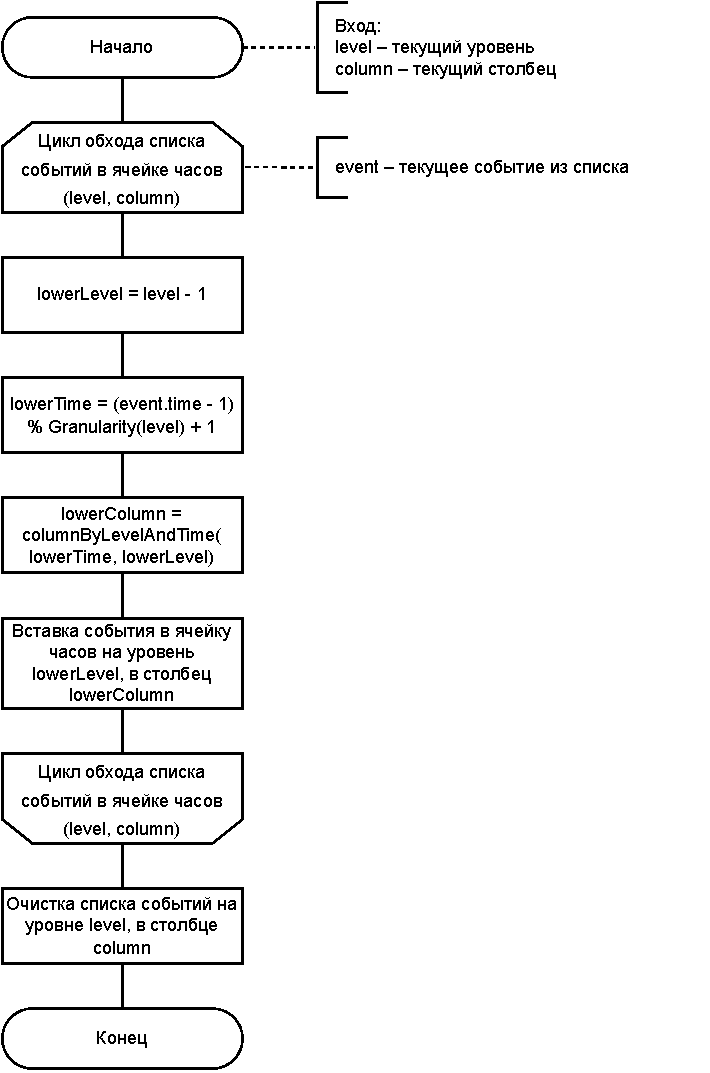
\includegraphics[width=0.8\columnwidth]{inc/img/hybrid_moveEvents_schema.pdf}
	\caption{Схема алгоритма перемещения событий из ячейки часовой структуры на уровень ниже}
	\label{img:hybrid_moveEvents_schema}	
\end{figure}

\clearpage
На рисунке \ref{img:hybrid_processEvent_schema} представлена схема алгоритма обработки одного события.
\begin{figure}[h!btp]
	\centering
	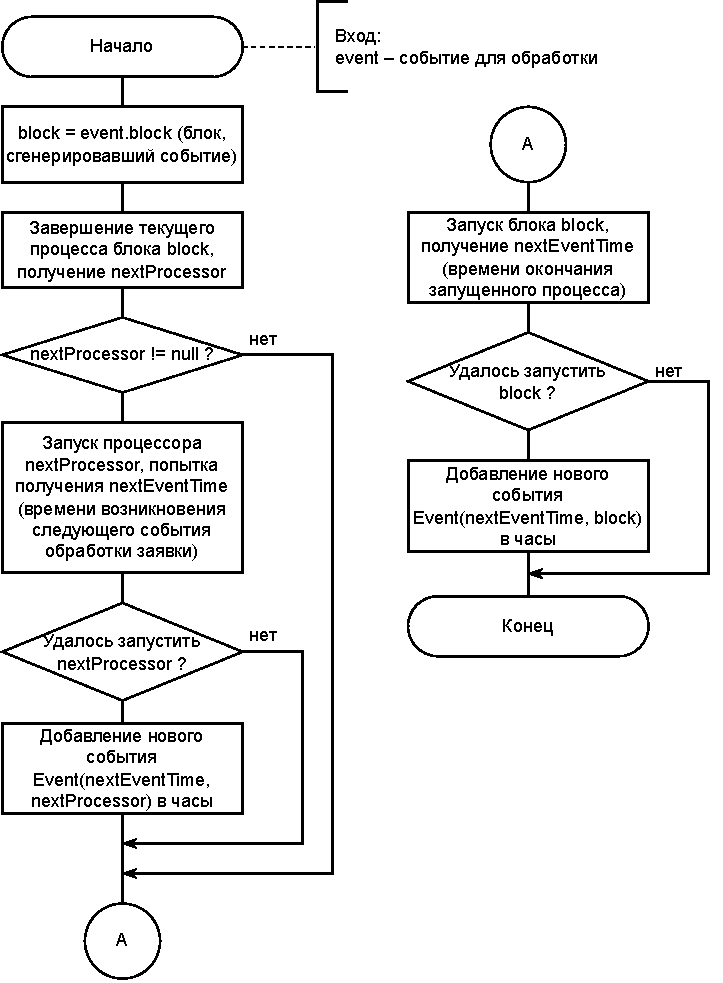
\includegraphics[width=0.8\columnwidth]{inc/img/hybrid_processEvent_schema.pdf}
	\caption{Схема алгоритма обработки одного события}
	\label{img:hybrid_processEvent_schema}	
\end{figure}

\clearpage
\section{Пошаговый алгоритм}
Пошаговый алгоритм подробно описан в соответствующем пункте аналитического раздела. 

Схема пошагового алгоритма представлена на рисунке \ref{img:delta_t_schema}.

\begin{figure}[h!btp]
	\centering
	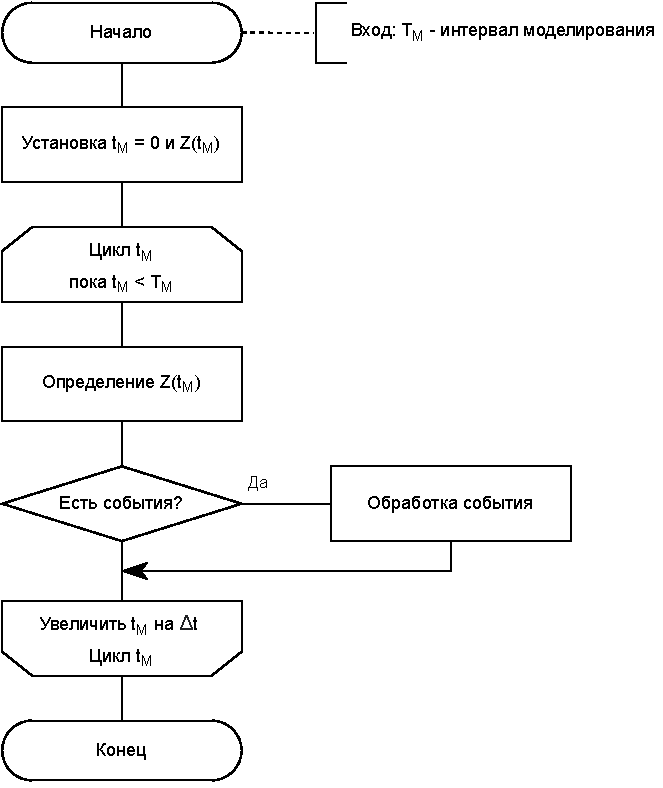
\includegraphics[width=0.8\columnwidth]{inc/img/delta_t_schema.pdf}
	\caption{Схема пошагового алгоритма}
	\label{img:delta_t_schema}	
\end{figure}

Используемые обозначения:
\begin{itemize}
	\item $t_M$ --- текущее значение модельного времени;
	\item $Z(t_M)$ --- состояние системы в текущий момент времени;
	\item $T_M$ --- интервал моделирования.
\end{itemize}

\section{Событийный алгоритм}
Событийный алгоритм подробно описан в соответствующем пункте аналитического раздела. 

Схема событийного алгоритма представлена на рисунке \ref{img:delta_z_schema}.

\begin{figure}[h!btp]
	\centering
	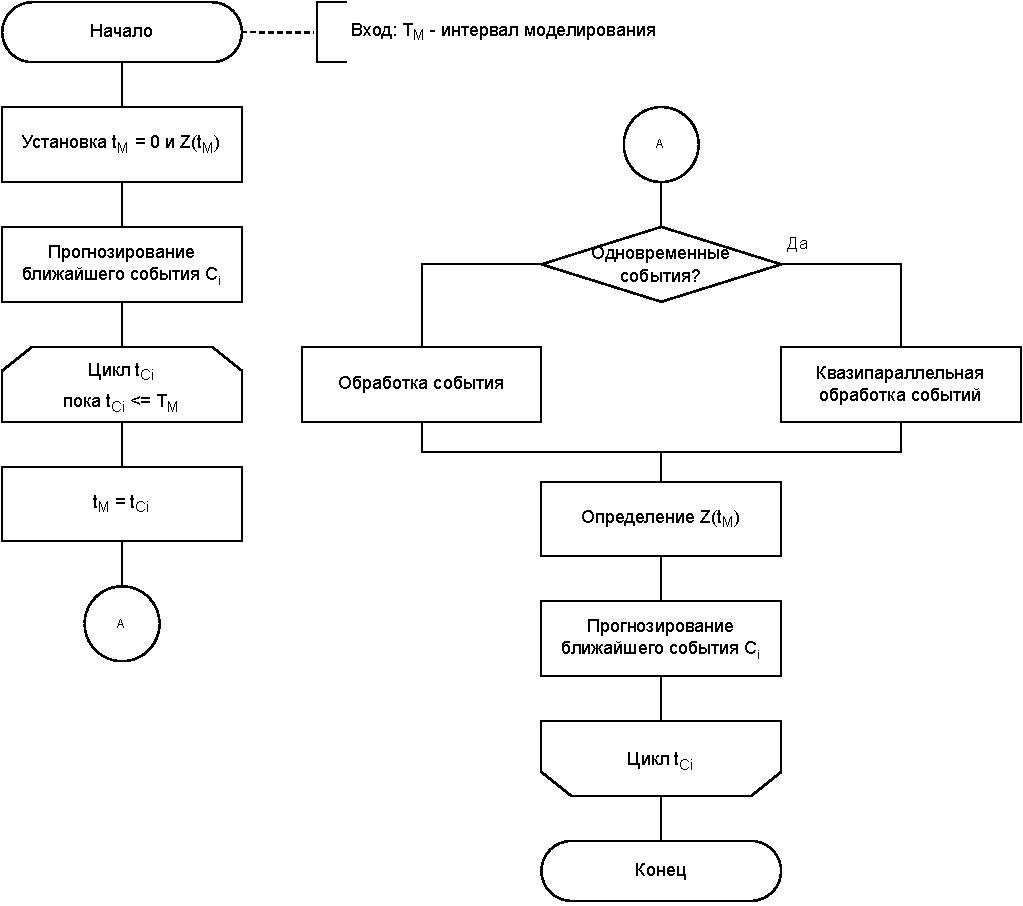
\includegraphics[width=1\columnwidth]{inc/img/delta_z_schema.pdf}
	\caption{Схема событийного алгоритма}
	\label{img:delta_z_schema}	
\end{figure}

Используемые обозначения:
\begin{itemize}
	\item $t_M$ --- текущее значение модельного времени;
	\item $Z(t_M)$ --- состояние системы в текущий момент времени;
	\item $T_M$ --- интервал моделирования;
	\item $t_{соб i}$ --- время возникновения $i$-го события.
\end{itemize}

\section{Моделируемая СМО}
В качестве моделируемой системы предлагается рассмотреть модель МФЦ.

Согласно информации, предоставленной официальным сайтом мэра Москвы \cite{mos_ru}, наименее загруженными днями для МФЦ считаются выходные, а максимальная загрузка приходится на вторник. В будние дни наименьшая загрузка наблюдается с 08.00 до 11.00 и с 14.00 до 20.00. Время работы МФЦ --- с 08.00 до 20.00 без перерывов и выходных. Среднее время ожидания приема в центрах госуслуг составляет 3 минуты, максимальное --- 15 минут.

Согласно статье с сайте Портала Правительства Московской области \cite{mosreg_ru} количество окон обслуживания в одном из подмосковных МФЦ было увеличено до 30.

Тогда моделируемая система будет состоять из:
\begin{enumerate}
	\item Автоматов с талонами (4 шт). Время подбора и получения талона клиентом на каждом автомате составляет $15\pm60$ секунд.
	\item Окон обслуживания (до 40 шт). Время обслуживания одного клиента в окне составляет от $10$  до $30$ минут.
	\item Работников архива (10 чел). После обслуживания клиента в одном из окон, информация о предоставленной услуге вместе с данными о нужных документах заносится в систему одним из работников архива. Длительность этого процесса зависит от оказываемой услуги и количества документов, необходимых для подготовки, ввиду чего время обслуживания обладает большим разбросом и может занимать от $5$ до $20$ минут.
\end{enumerate}

Необходимо смоделировать работу такого МФЦ в течение одной недели.


За минимальный шаг времени принимается 1 секунда. Тогда общее время моделирования для 7 12-часовых рабочих дней эквивалентно 302400 секундам. Пиковые интервалы приходятся на время с 11.00 до 14.00, т.е. их длина составляет 10800 секунд (3 часа), а непиковые интервалы приходятся на оставшиеся 9 часов рабочего дня с общей длительностью в 32400 секунды. Ввиду отсутствия в открытом виде статистической выборки по посещаемости МФЦ среднее время появление нового посетителя будем считать 30 секунд для пикового интервала и 420 секунд (7 минут) для непикового. Появление посетителей подчинено экспоненциальному закону.

На рисунке \ref{img:system_modelling_distr}	 представлено распределение для генератора заявок, созданное на основе предоставленной информации о загруженности МФЦ.

\begin{figure}[h!btp]
	\centering
	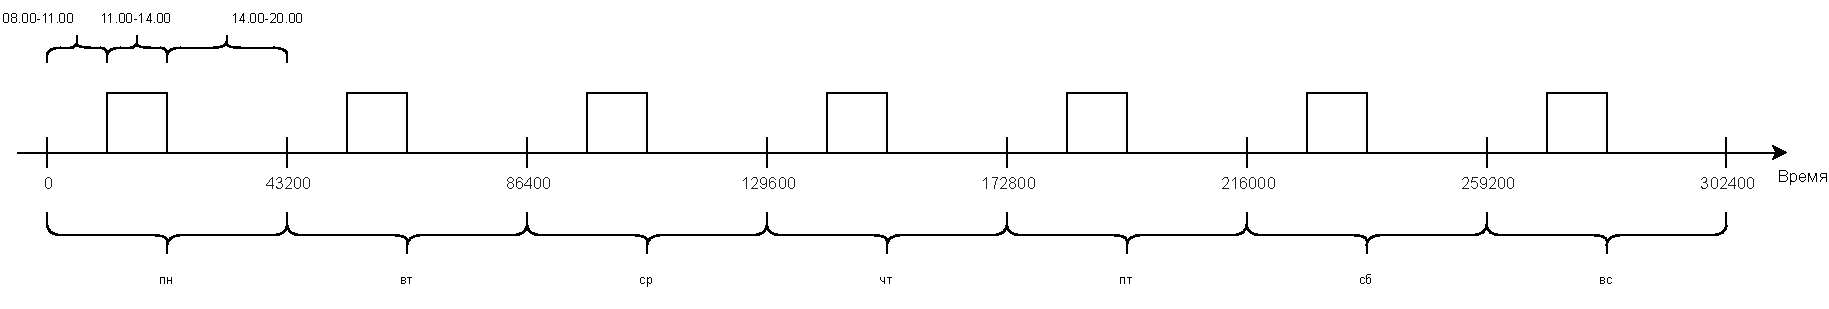
\includegraphics[width=1\columnwidth]{inc/img/system_modelling_distr.pdf}
	\caption{Распределение событий поступления заявок в МФЦ}
	\label{img:system_modelling_distr}	
\end{figure}

На рисунке \ref{img:system_modelling} представлена схема МФЦ в терминах СМО.

\begin{figure}[h!btp]
	\centering
	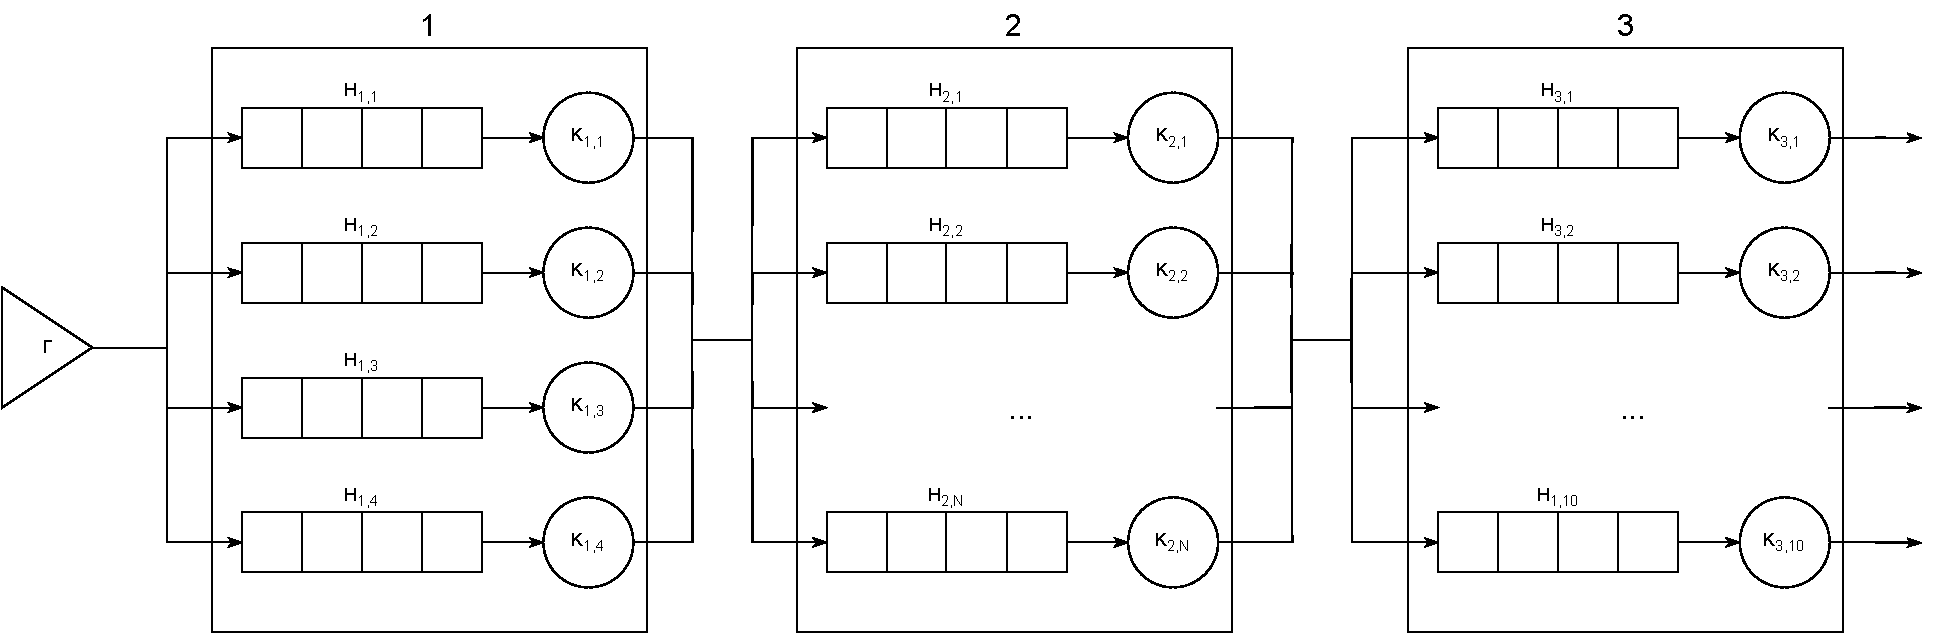
\includegraphics[width=1\columnwidth]{inc/img/system_modelling.pdf}
	\caption{Схема МФЦ в терминах СМО}
	\label{img:system_modelling}	
\end{figure}

	
\section{Выводы}
В рамках данного раздела были описаны основные особенности разрабатываемого комбинированного алгоритма продвижения модельного времени. Были изложены ключевые этапы комбинированного, а также пошагового и событийного алгоритмов в виде схем алгоритмов. Также были описаны требования к моделируемой в рамках данной работы системы массового обслуживания.